\newcommand\tab[1][0,4cm]{\hspace*{#1}}
\newcommand\longtab[1][1cm]{\hspace*{#1}}

\chapter{Généralités}
\section{Introduction au sujet}

\paragraph*{}
Ces dernières années, la communauté des lecteurs algériens a connu une croissance rapide et le taux de participation aux salons du livre est prometteur. Avec cette quantité de livres achetés, de nouveaux problèmes voient le jour, en plus des problèmes déjà existants tels que: les prix relativement élevés de certains livres, la rareté de certains autres et la tâche difficile que les lecteurs doivent endurer pour s'identifier avec d'autres membres de la communauté qui partage les mêmes intérêts et se localisant dans la même zone géographique, se pose le problème de stockage de ces livres et du fait qu’ils peuvent être mieux traités par un nouveau lecteur que de prendre de la place sur une étagère quelque part.


\paragraph*{}
Il existe des clubs de lecture et des réunions sociales où les gens échangent, vendent, donnent des livres et même rencontrent de nouvelles personnes, ce qui laisse penser qu'il existe un groupe de personnes qui:

\begin{list}{•}{}
\item Ont des livres.
\item Sont disposés à abandonner les livres déjà lus.
\item Veulent économiser de l’argent tout en faisant lire des livres
\end{list}

\paragraph*{}
Comme nous venons de le dire, certaines solutions existent pour cette communauté et nous en explorerons certaines dans les sections suivantes tout en soulignant leurs lacunes et en expliquant comment une fenêtre d'opportunités est encore ouverte pour résoudre le problème une fois pour toutes.
\newpage

\section{Solutions déjà existents}

\subsection{Non technologique}

\paragraph*{}
L'analyse de cette question donnera lieu à deux concepts intéressants qui existent déjà et qui sont, dans une certaine mesure, fonctionnels:\\\\
\textbf{1. Événements d'échange de livres}\\
\tab Certains clubs de lecture et cafés organisent des événements où les participants sont invités à apporter les livres qu'ils souhaitent transmettre aux autres lecteurs et à en obtenir de nouveaux dans une atmosphère conviviale.

\subparagraph*{}
\begin{list}{•}{\textbf{Avantages}}
\item Les participants peuvent vivre toute l'expérience humaine d'échanger un livre.
\item Les participants sont à découvrir de nouveaux livres par des personnes autres que des simple avis en ligne.
\item Les participants établissent des liens significatifs avec leurs collègues lecteurs de livres.
\end{list}

\subparagraph*{}
\begin{list}{•}{\textbf{Inconvénients}}
\item De tels événements durent au mieux 2 jours, ce qui fait que beaucoup de gens ratent l'occasion.
\item En raison de la limitation géographique, de tels événements ne peuvent être accessibles que par quelques résidents proches de la région.
\item coûteux en terme de temps investi.\\
\end{list}

\textbf{2. Échanges informels de livres}\\
\tab Certains échanges de livres sont informels - une étagère ou une boîte est fournie où les livres peuvent être laissés ou ramassés. L'échange repose sur les utilisateurs qui sortent et prennent des livres et n'est généralement pas supervisé.\\
\tab C'est une pratique courante dans les auberges de jeunesse où les voyageurs peuvent laisser un livre et emporter un livre différent avec eux. Certaines gares ferroviaires en Grande-Bretagne ont des échanges de livres informels et une a également été installée dans une cabine téléphonique à Kington Magna.

\subparagraph*{}
\begin{list}{•}{\textbf{Avantages}}
\item Le processus est très rapide et pratiquement pas de temps perdu.
\item Absence de limite de temps, ils peuvent être échangés à tout moment.
\end{list}

\subparagraph*{}
\begin{list}{•}{\textbf{Inconvénients}}
\item Le besoin de donateurs au début du projet.
\item L'absence d'un système de contrôle de qualité pour les livres mis contre les prises.
\end{list}
\newpage

\subsection{Technologique}

\paragraph*{}
Il existe plusieurs sites Web et très peu d'applications populaires offrant le type de bonne expérience présente de manière traditionnelle, nous allons explorer certaines des plus populaires solutions existant aujourd’hui.\\

{\large \textbf{\\1. BookMooch:\\}}

\begin{wrapfigure}[15]{r}{3cm}

\includegraphics[width=4cm]{Images/chapter1/bookMoochLogo.jpg}
\caption{BookMooch logo}
\end{wrapfigure}
\tab Portant bien son nom, avec le fameux slogan ​“Give books away, Get books you want”,BookMooch est une société de publication delivres en ligne par laquelle ses membres peuventéchanger des livres entre eux. Son fondateur,
John Buckman, a choisi ce nom pour l'entrepriseen référence à l'acte de donner un livre sansattendre de le récupérer. Les utilisateurs, alors, sont considérés comme des BookMoochers etbénéficient à bien des égards de ce systèmecommercial unique.\\
\tab En bref, les utilisateurs «achètent» les livres des autres membres	en utilisant uniquement des points. Chaque membre peut accumuler des points en soumettant les titres des livres qu'il veut donner et en envoyant ses livres à d'autres utilisateurs. Avec suffisamment de points, ils peuvent alors commencer à recevoir les titres d'autres personnes, et le processus continue à partir de là. Le seul coût pour les membres est celui de l'envoi des livres qu'ils envoient à d'autres.\\

\subparagraph*{}
\begin{list}{•}{\textbf{Avantages}}
\item L'adhésion à cette entreprise est gratuite.
\item Vous pouvez choisir parmi une grande variété de livres.
\item Une liste de souhaits connectée à amazon où vous recevrez des notifications lorsque des livres sont disponibles.
\end{list}

\subparagraph*{}
\begin{list}{•}{\textbf{Inconvénients}}
\item Pour recevoir, il faut donner.
\item Dans une certaine mesure, la plate-forme peut être un terrain de jeu pour les fraudeurs.
\item La plate-forme n'exploite pas l'emplacement des membres.
\end{list}
\newpage

{\large \textbf{2. Bookup:\\}}

\tab L'application Bookup est destinée aux lecteurs de livres imprimés qui souhaitent échanger leurs livres contre d'autres livres de leur région, gratuitement, et éventuellement se faire un nouvel ami partageant le même intérêt pour la lecture. Bookup fournit une fonctionnalité d’échange de livre en fonction de l’emplacement.
\begin{figure}[h]
\begin{center}
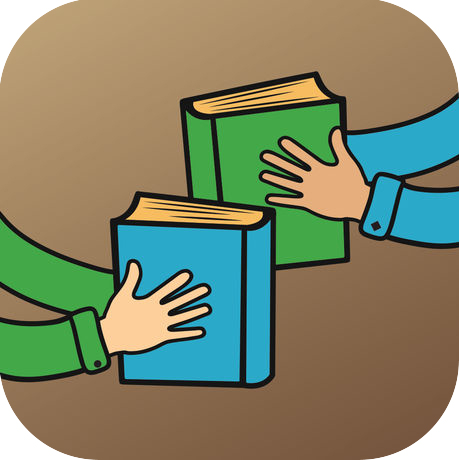
\includegraphics[width=2.5cm]{Images/chapter1/bookUpLogo.jpg}
\caption{Bookup logo}
\end{center}
\end{figure}

\subparagraph*{}
\begin{list}{•}{\textbf{Avantages}}
\item La plate-forme exploite pas l'emplacement des membres.
\item Fonction de bibliothèque personnelle que vous pouvez personnaliser à votre guise.
\item Liberté absolue pour les utilisateurs de discuter en temps réel et de trouver un moyen d'exécuter l'échange.
\item Un mécanisme simple d'exploration aléatoire de livres proches.
\end{list}

\subparagraph*{}
\begin{list}{•}{\textbf{Inconvénients}}
\item L'application est disponible uniquement sur les appareils Apple.
\item une expérience utilisateur moyenne.
\item Un manque évident d'informations sur les livres et les utilisateurs.
\end{list}

\begin{figure}[h]
\begin{center}
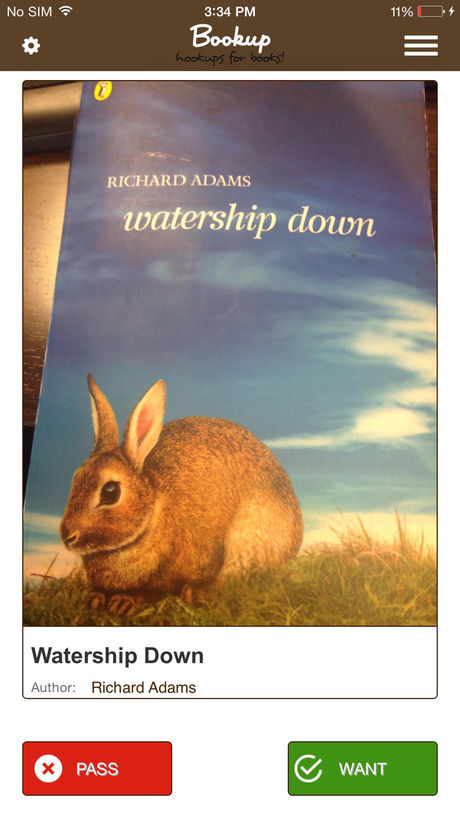
\includegraphics[width=2.5cm]{Images/chapter1/bookUpScreenshot.jpg}
\caption{Mecanisme de suggestion de Bookup}
\end{center}
\end{figure}
